\documentclass{article}
\usepackage[utf8]{inputenc}
\usepackage[margin=0.8in]{geometry}
\usepackage{graphicx}
\usepackage{algorithm}
\usepackage{algorithmicx}
\usepackage[noend]{algpseudocode}

\usepackage{tikz}

\definecolor{myseagreen}{RGB}{88,197,191}
\definecolor{mysalmon}{RGB}{255,160,122}
\definecolor{myred}{RGB}{255,102,102}
\definecolor{mypurple}{RGB}{225,145,255}
\definecolor{myblack}{RGB}{0,0,0}
\definecolor{mywhite}{RGB}{255,255,255}

% for black and white printing
\definecolor{myseagreen}{rgb}{1.0,1.0,1.0}
\definecolor{mysalmon}{rgb}{1.0,1.0,1.0}
\definecolor{myred}{rgb}{1.0,1.0,1.0}
\definecolor{mypurple}{rgb}{1.0,1.0,1.0}

\usepackage{tikz}

\usetikzlibrary{calc,shapes.multipart,chains,arrows,positioning}

\tikzstyle{vertex}=[draw,fill=myseagreen,circle,minimum size=24pt,inner sep=0pt]

\tikzstyle{splitvertex}=[draw,fill=myseagreen,circle split,minimum size=24pt]

\usetikzlibrary{
  shapes.multipart,
  matrix,
  positioning,
  shapes.callouts,
  shapes.arrows,
  shapes.geometric,
  decorations.shapes,
  shapes,
  fit,
  arrows,
  positioning,
  trees,
  mindmap,
  calc}

% START OF DOCUMENT %
\title{Basic Graph Theory}
\author{Jongwan Kim}
\date{28 September 2018}

\begin{document}

\maketitle

\section{What is a Graph?}
A graph is a set of nodes that are connected together by edges. Graphs are used to represent a variety of computer science problems. For example, we can generate a graph with airports and draw lines between each airport to indicate flight paths. This structure can be used to solve problems such as connectivity and shortest path. When using big O notation, instead of $n$, we use $E$ and $V$ to represent edges and vertices, which are nodes, respectively.

\begin{figure} [H]
    \begin{center}
        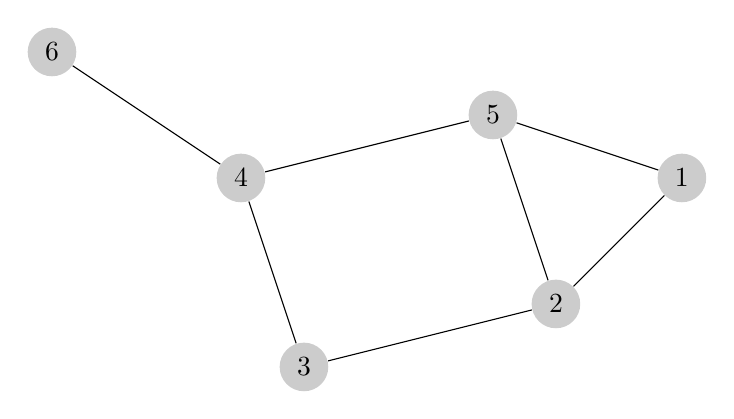
\begin{tikzpicture}
          [scale=.8,auto=left,every node/.style={circle,fill=black!20}]
          \node (n6) at (1,10) {6};
          \node (n4) at (4,8)  {4};
          \node (n5) at (8,9)  {5};
          \node (n1) at (11,8) {1};
          \node (n2) at (9,6)  {2};
          \node (n3) at (5,5)  {3};
        
          \foreach \from/\to in {n6/n4,n4/n5,n5/n1,n1/n2,n2/n5,n2/n3,n3/n4}
            \draw (\from) -- (\to);
        \end{tikzpicture}
    \end{center}
    \caption{Example of a graph}
\end{figure}

\subsection{Undirected Graphs}
Undirected graphs consist of a series of nodes with line segments in between them. These line segments, called edges, determine which nodes are connected. In an undirected graph, if vertices $u$ and $v$ are connected by an edge, then a traversal can be made in both ways. In other words, one can go from $u$ to $v$ and from $v$ to $u$. When a problem statements says "graphs with bidirectional edges" or something of that sort, you can interpret it as an undirected graph because bidirected graphs and undirected graphs basically have same properties.

\subsection{Directed Graphs}
Certain graphs only allow for one way movement. We call these graphs directed graphs. Typically, when we draw a graph, we place all of the nodes and then draw line segments in between the points. In a directed graph, these line segments are turned into rays that represent movement. If a directed graph has a path that allows two-way movement, then we draw arrows on both end of the line segment.

\subsection{Weighted Graphs}
In most cases, we often give some weight to each edge. This weight represents the value associated with it. For example, in the case of creating an airplane network, we know that going from DC to LA is much further than DC to NYC. Therefore, we can give each line segment a different weight, such as the distance, to represent the value of each edge.

\section{Searches}
Often, we want to navigate through these graphs to look for a specific thing. To do this, we have two primary approaches: breadth first search (BFS) and depth first search (DFS).

\subsection{BFS}
The first approach we use is searching by breadth. At each node, we recursively call each of its neighbors, expanding outward. This way, our region of inspection expands our circularly and fairly evenly. Essentially, its as if at each fork in the graph, we clone ourselves and one clone goes down each direction. This is very useful expanding out steadily and making sure we don't skip over regions.

\subsection{DFS}
Another approach that is used is by searching by depth. At each node, we simply pick one direction and keep following this path all the way down till we hit a base case. Then we trek back to the last fork in the road and take that path till we hit a base case. This continues till the objective is reached or the entire graph is traversed. In some cases, this can be more effective, however it risks the fallacy of skipping over potentially very rewarding nodes that are very close simply because they aren't explored early on.

\section{Shortest Path}

We want to find the shortest path between any two points. We consider that each edge has some weight or penalty to traverse. This weight represents the cost needed to traverse the connection. This graph can be either directed or undirected.

\subsection{Dijkstra}

Dijkstra's algorithm is a common approach to finding the shortest path between any two points. This is done through a greedy approach. 

For every vertex $v$ in the graph, we keep track of the shortest known distance $dist(v)$ from the source to $v$, a boolean $visited(v)$ to keep track of which nodes we ``visited,'' and a pointer to the previous node in the shortest known path $prev(v)$ so that we can trace the shortest path once the algorithm finishes.

Dijkstra iteratively ``visits'' the next nearest vertex, updating the distances to that vertex's neighbors if necessary. The nearest vertex is simply the one that is closest to what we have already explored, aka has the lowest weight on its edge.

\begin{algorithm}[H]
\caption{Dijkstra}
\begin{algorithmic}
\ForAll{vertices $v$}
	\State $dist(v) \gets \infty$
	\State $visited(v) \gets 0$
    \State $prev(v) \gets -1$
\EndFor
\State $dist(src) \gets 0$
\While{$\exists v$ s.t. $visited(v)=0$}
	\State $v \equiv v$ s.t. $visited(v)=0$ with min $dist(v)$
    \State $visited(v) \gets 1$
	\ForAll{neighbors $u$ of $v$}
    	\If{$visited(u) = 0$}
    		\State $alt \gets dist(v) + weight(v, u)$
			\If{$alt < dist(u)$}
				\State $dist(u) \gets alt$
   	        	\State $prev(u) \gets v$
			\EndIf
        \EndIf
    \EndFor
\EndWhile
\end{algorithmic}
\end{algorithm}

\begin{center}
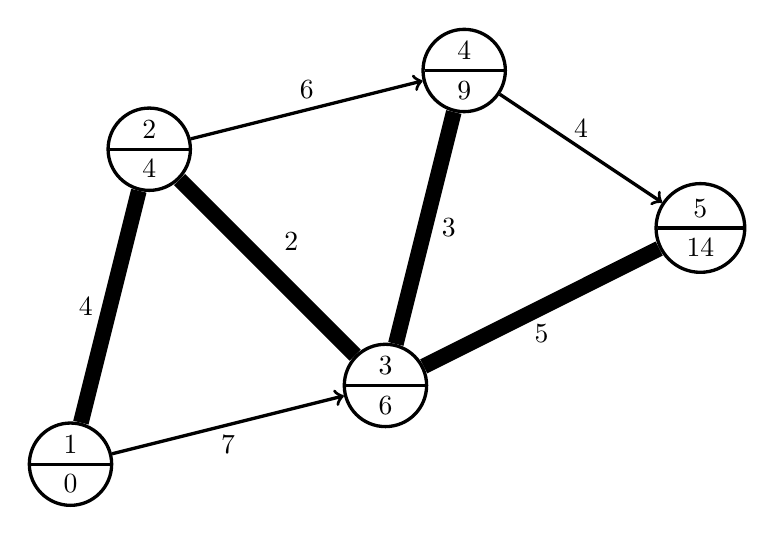
\begin{tikzpicture}[very thick,edge from parent/.style={draw,<-},level/.style={sibling distance=30mm/#1}]
\draw (0, 0) node [splitvertex, fill=myred] (v1) {1\nodepart{lower}0};
\draw (1, 4) node [splitvertex, fill=myred] (v2) {2\nodepart{lower}4};
\draw (4, 1) node [splitvertex, fill=myred] (v3) {3\nodepart{lower}6};
\draw (5, 5) node [splitvertex, fill=myred] (v4) {4\nodepart{lower}9};
\draw (8, 3) node [splitvertex, fill=myred] (v5) {5\nodepart{lower}14};
\draw[line width=2mm] (v1) -- (v2) node[midway, left] {4};
\draw[line width=2mm] (v2) -- (v3) node[midway, above right] {2};
\draw[->] (v1) -- (v3) node[midway, below] {7};
\draw[->] (v2) -- (v4) node[midway, above] {6};
\draw[line width=2mm] (v3) -- (v4) node[midway, right] {3};
\draw[line width=2mm] (v3) -- (v5) node[midway, below] {5};
\draw[->] (v4) -- (v5) node[midway, above] {4};
\end{tikzpicture}
\end{center}

\subsection{Bellman-Ford}

Bellman-Ford is a single-source $O(VE)$ shortest path algorithm that works when edge weights can be negative. The key observation here is that the shortest path, assuming no negative cycles, has length at most $V-1$.  If we loop over all edges and consider if they form a new shortest path to their endpoint we can find all shortest paths of length 1.  If we repeat this loop $V-1$ times we discover all paths of length up to $V-1$. To detect a negative cycle we simply run the loop one last time.  If any shorter paths are discovered, then the optimal path is longer than $V-1$ nodes.  The only way this is possible is if there is a negative cycle.

\begin{algorithm}[H]
\caption{Bellman-Ford}
\begin{algorithmic}
\ForAll{vertices $v$}
	\State $dist(v)\gets\infty$
    \State $prev(v)\gets -1$
\EndFor
\State $dist(src) \gets 0$
\For{$i=1$ to $V-1$}
	\ForAll{edges $(u,v)$}
		\If{$dist(u)+weight(u,v) < dist(v)$}
    	    \State $dist(v) \gets dist(u)+weight(u,v)$
	        \State $prev(v) \gets u$
        \EndIf
	\EndFor
\EndFor
\ForAll{edges $(u,v)$}
	\Comment{check for negative cycles}
	\If{$dist(u)+weight(u,v) < dist(v)$}
   	    \State{negative cycle detected}
	\EndIf
\EndFor
\end{algorithmic}
\end{algorithm}

\subsection{Floyd-Warshall}
Floyd-Warshall solves the shortest path problem for all pairs of vertices in $O(V^3)$ time, which is faster than $V$ single-source Dijkstra runs on a dense graph. Floyd-Warshall works even if some edge weights are negative but not if the graph has a negative cycle. Essentially, it computes the path from every node to every node.

\begin{algorithm}[H]
\caption{Floyd-Warshall}
\begin{algorithmic}
\ForAll{vertices $v$}
	\State $dist(v,v)=0$
\EndFor
\ForAll{edges $(u,v)$}
	\State $dist(u,v)=weight(u,v)$
\EndFor
\ForAll{vertices $k$}
	\ForAll{vertices $i$}
    	\ForAll{vertices $j$}
        	\If{$dist(i,j) > dist(i,k)+dist(k,j)$}
            	\State $dist(i,j) \gets dist(i,k)+dist(k,j)$
            \EndIf
        \EndFor
    \EndFor
\EndFor
\end{algorithmic}
\end{algorithm}

\end{document}
